\documentclass{standalone}
\usepackage{tikz}
\usetikzlibrary{patterns, positioning}


\begin{document}
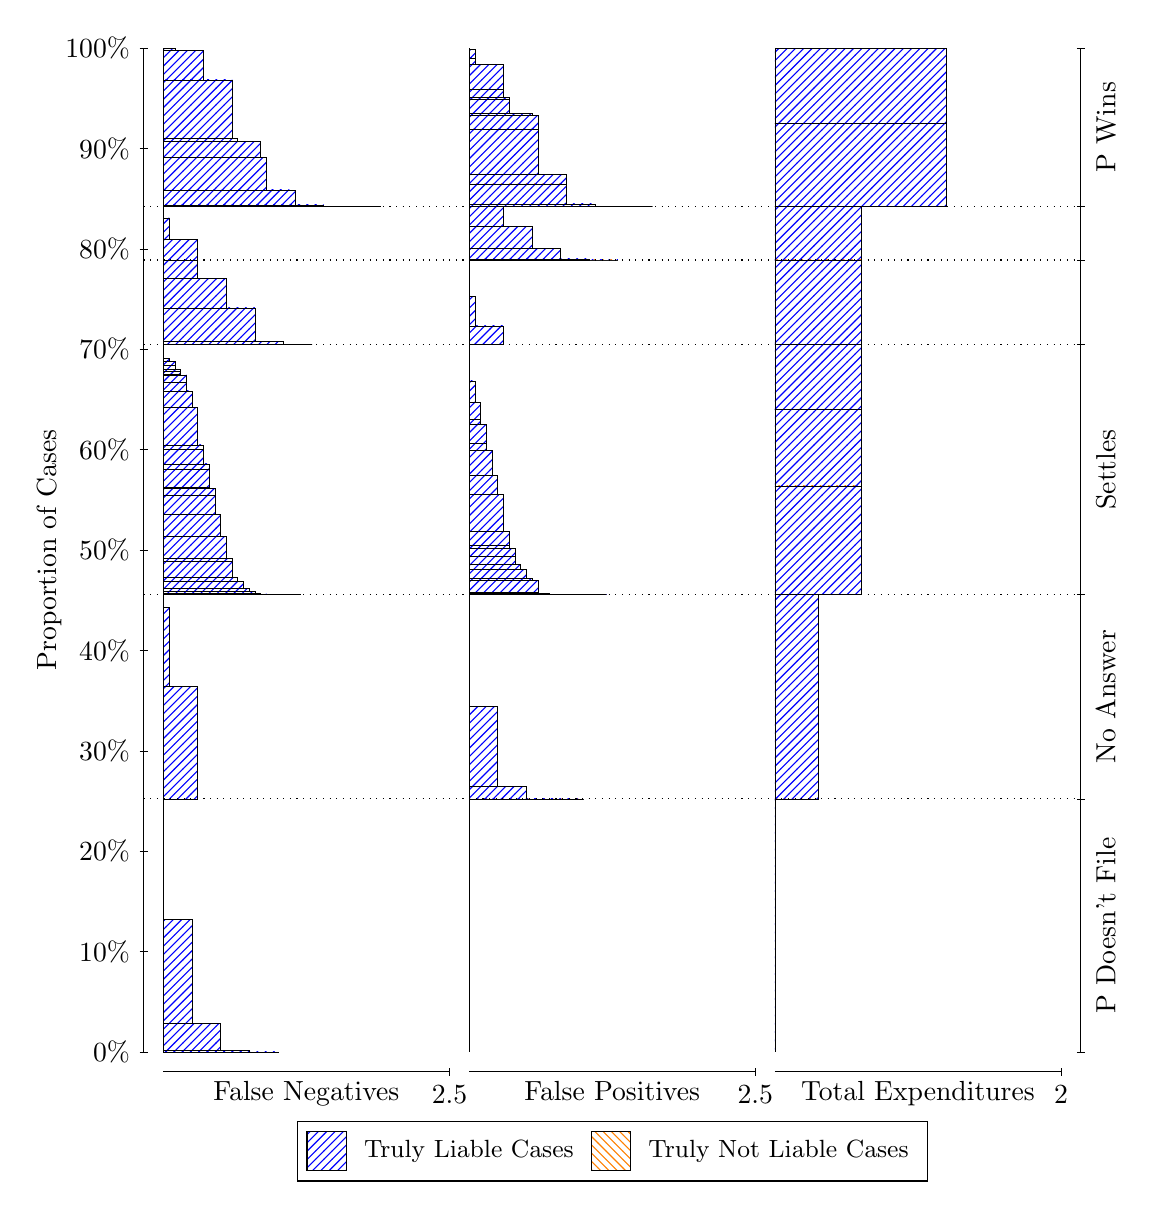
\begin{tikzpicture}
\draw[black, very thin] (1.5,1.75) -- (1.5,14.5);
\node[rotate=90, text=black, anchor=center] at (0.3, 8.125) {Proportion of Cases};
\draw[black, very thin] (1.45,1.75) -- (1.55,1.75);
\node[text=black, anchor=east] at (1.45, 1.75) {0\%};
\draw[black, very thin] (1.45,3.025) -- (1.55,3.025);
\node[text=black, anchor=east] at (1.45, 3.025) {10\%};
\draw[black, very thin] (1.45,4.3) -- (1.55,4.3);
\node[text=black, anchor=east] at (1.45, 4.3) {20\%};
\draw[black, very thin] (1.45,5.575) -- (1.55,5.575);
\node[text=black, anchor=east] at (1.45, 5.575) {30\%};
\draw[black, very thin] (1.45,6.85) -- (1.55,6.85);
\node[text=black, anchor=east] at (1.45, 6.85) {40\%};
\draw[black, very thin] (1.45,8.125) -- (1.55,8.125);
\node[text=black, anchor=east] at (1.45, 8.125) {50\%};
\draw[black, very thin] (1.45,9.4) -- (1.55,9.4);
\node[text=black, anchor=east] at (1.45, 9.4) {60\%};
\draw[black, very thin] (1.45,10.675) -- (1.55,10.675);
\node[text=black, anchor=east] at (1.45, 10.675) {70\%};
\draw[black, very thin] (1.45,11.95) -- (1.55,11.95);
\node[text=black, anchor=east] at (1.45, 11.95) {80\%};
\draw[black, very thin] (1.45,13.225) -- (1.55,13.225);
\node[text=black, anchor=east] at (1.45, 13.225) {90\%};
\draw[black, very thin] (1.45,14.5) -- (1.55,14.5);
\node[text=black, anchor=east] at (1.45, 14.5) {100\%};

\draw[black, very thin] (13.4,1.75) -- (13.4,14.5);
\draw[black, very thin] (13.35,1.75) -- (13.45,1.75);
\node[anchor=west] at (13.35, 1.75) {};
\draw[black, very thin] (13.35,4.964) -- (13.45,4.964);
\node[anchor=west] at (13.35, 4.964) {};
\draw[black, very thin] (13.35,7.5596) -- (13.45,7.5596);
\node[anchor=west] at (13.35, 7.5596) {};
\draw[black, very thin] (13.35,10.736) -- (13.45,10.736);
\node[anchor=west] at (13.35, 10.736) {};
\draw[black, very thin] (13.35,11.808) -- (13.45,11.808);
\node[anchor=west] at (13.35, 11.808) {};
\draw[black, very thin] (13.35,12.488) -- (13.45,12.488);
\node[anchor=west] at (13.35, 12.488) {};
\draw[black, very thin] (13.35,14.5) -- (13.45,14.5);
\node[anchor=west] at (13.35, 14.5) {};

\draw[black, very thin, pattern color=blue, pattern=north east lines] (1.75,1.75) rectangle (3.2033,1.7502);
\draw[black, very thin, pattern color=blue, pattern=north east lines] (1.75,1.7502) rectangle (2.84,1.7745);
\draw[black, very thin, pattern color=blue, pattern=north east lines] (1.75,1.7745) rectangle (2.4767,2.1146);
\draw[black, very thin, pattern color=blue, pattern=north east lines] (1.75,2.1146) rectangle (2.1133,3.4294);
\draw[black, very thin, pattern color=orange, pattern=north west lines] (1.75,3.4294) rectangle (1.75,3.4294);
\draw[black, very thin, pattern color=blue, pattern=north east lines] (1.75,3.4294) rectangle (1.75,4.964);
\draw[black, very thin, pattern color=blue, pattern=north east lines] (1.75,4.964) rectangle (2.186,6.3896);
\draw[black, very thin, pattern color=blue, pattern=north east lines] (1.75,6.3896) rectangle (1.8227,7.4005);
\draw[black, very thin, pattern color=orange, pattern=north west lines] (1.75,7.4005) rectangle (1.75,7.4005);
\draw[black, very thin, pattern color=blue, pattern=north east lines] (1.75,7.4005) rectangle (1.75,7.5596);
\draw[black, very thin, pattern color=blue, pattern=north east lines] (1.75,7.5596) rectangle (3.494,7.5597);
\draw[black, very thin, pattern color=blue, pattern=north east lines] (1.75,7.5597) rectangle (3.3487,7.5597);
\draw[black, very thin, pattern color=blue, pattern=north east lines] (1.75,7.5597) rectangle (3.2033,7.5629);
\draw[black, very thin, pattern color=blue, pattern=north east lines] (1.75,7.5629) rectangle (3.1307,7.5653);
\draw[black, very thin, pattern color=blue, pattern=north east lines] (1.75,7.5653) rectangle (3.058,7.5654);
\draw[black, very thin, pattern color=blue, pattern=north east lines] (1.75,7.5654) rectangle (3.058,7.5686);
\draw[black, very thin, pattern color=blue, pattern=north east lines] (1.75,7.5686) rectangle (2.9853,7.5731);
\draw[black, very thin, pattern color=blue, pattern=north east lines] (1.75,7.5731) rectangle (2.9127,7.6037);
\draw[black, very thin, pattern color=blue, pattern=north east lines] (1.75,7.6037) rectangle (2.84,7.6423);
\draw[black, very thin, pattern color=blue, pattern=north east lines] (1.75,7.6423) rectangle (2.7673,7.7235);
\draw[black, very thin, pattern color=blue, pattern=north east lines] (1.75,7.7235) rectangle (2.6947,7.7297);
\draw[black, very thin, pattern color=blue, pattern=north east lines] (1.75,7.7297) rectangle (2.6947,7.7749);
\draw[black, very thin, pattern color=blue, pattern=north east lines] (1.75,7.7749) rectangle (2.622,7.9777);
\draw[black, very thin, pattern color=blue, pattern=north east lines] (1.75,7.9777) rectangle (2.622,8.0227);
\draw[black, very thin, pattern color=blue, pattern=north east lines] (1.75,8.0227) rectangle (2.5493,8.2999);
\draw[black, very thin, pattern color=blue, pattern=north east lines] (1.75,8.2999) rectangle (2.4767,8.5758);
\draw[black, very thin, pattern color=blue, pattern=north east lines] (1.75,8.5758) rectangle (2.404,8.8192);
\draw[black, very thin, pattern color=blue, pattern=north east lines] (1.75,8.8192) rectangle (2.404,8.9061);
\draw[black, very thin, pattern color=blue, pattern=north east lines] (1.75,8.9061) rectangle (2.3313,8.9225);
\draw[black, very thin, pattern color=blue, pattern=north east lines] (1.75,8.9225) rectangle (2.3313,9.1489);
\draw[black, very thin, pattern color=blue, pattern=north east lines] (1.75,9.1489) rectangle (2.3313,9.2194);
\draw[black, very thin, pattern color=blue, pattern=north east lines] (1.75,9.2194) rectangle (2.2587,9.4033);
\draw[black, very thin, pattern color=blue, pattern=north east lines] (1.75,9.4033) rectangle (2.2587,9.4611);
\draw[black, very thin, pattern color=blue, pattern=north east lines] (1.75,9.4611) rectangle (2.186,9.936);
\draw[black, very thin, pattern color=blue, pattern=north east lines] (1.75,9.936) rectangle (2.1133,10.147);
\draw[black, very thin, pattern color=blue, pattern=north east lines] (1.75,10.147) rectangle (2.0407,10.252);
\draw[black, very thin, pattern color=blue, pattern=north east lines] (1.75,10.252) rectangle (2.0407,10.349);
\draw[black, very thin, pattern color=blue, pattern=north east lines] (1.75,10.349) rectangle (1.968,10.352);
\draw[black, very thin, pattern color=blue, pattern=north east lines] (1.75,10.352) rectangle (1.968,10.394);
\draw[black, very thin, pattern color=blue, pattern=north east lines] (1.75,10.394) rectangle (1.968,10.415);
\draw[black, very thin, pattern color=blue, pattern=north east lines] (1.75,10.415) rectangle (1.8953,10.473);
\draw[black, very thin, pattern color=blue, pattern=north east lines] (1.75,10.473) rectangle (1.8953,10.527);
\draw[black, very thin, pattern color=blue, pattern=north east lines] (1.75,10.527) rectangle (1.8227,10.562);
\draw[black, very thin, pattern color=orange, pattern=north west lines] (1.75,10.562) rectangle (1.75,10.562);
\draw[black, very thin, pattern color=blue, pattern=north east lines] (1.75,10.562) rectangle (1.75,10.736);
\draw[black, very thin, pattern color=blue, pattern=north east lines] (1.75,10.736) rectangle (3.6393,10.736);
\draw[black, very thin, pattern color=blue, pattern=north east lines] (1.75,10.736) rectangle (3.276,10.777);
\draw[black, very thin, pattern color=blue, pattern=north east lines] (1.75,10.777) rectangle (2.9127,11.2);
\draw[black, very thin, pattern color=blue, pattern=north east lines] (1.75,11.2) rectangle (2.5493,11.574);
\draw[black, very thin, pattern color=blue, pattern=north east lines] (1.75,11.574) rectangle (2.186,11.808);
\draw[black, very thin, pattern color=orange, pattern=north west lines] (1.75,11.808) rectangle (1.75,11.808);
\draw[black, very thin, pattern color=blue, pattern=north east lines] (1.75,11.808) rectangle (2.186,12.065);
\draw[black, very thin, pattern color=blue, pattern=north east lines] (1.75,12.065) rectangle (1.8227,12.342);
\draw[black, very thin, pattern color=orange, pattern=north west lines] (1.75,12.342) rectangle (1.75,12.342);
\draw[black, very thin, pattern color=blue, pattern=north east lines] (1.75,12.342) rectangle (1.75,12.488);
\draw[black, very thin, pattern color=blue, pattern=north east lines] (1.75,12.488) rectangle (4.5113,12.488);
\draw[black, very thin, pattern color=blue, pattern=north east lines] (1.75,12.488) rectangle (4.148,12.488);
\draw[black, very thin, pattern color=blue, pattern=north east lines] (1.75,12.488) rectangle (3.7847,12.509);
\draw[black, very thin, pattern color=blue, pattern=north east lines] (1.75,12.509) rectangle (3.712,12.509);
\draw[black, very thin, pattern color=blue, pattern=north east lines] (1.75,12.509) rectangle (3.4213,12.691);
\draw[black, very thin, pattern color=blue, pattern=north east lines] (1.75,12.691) rectangle (3.3487,12.698);
\draw[black, very thin, pattern color=blue, pattern=north east lines] (1.75,12.698) rectangle (3.058,13.109);
\draw[black, very thin, pattern color=blue, pattern=north east lines] (1.75,13.109) rectangle (2.9853,13.317);
\draw[black, very thin, pattern color=blue, pattern=north east lines] (1.75,13.317) rectangle (2.6947,13.348);
\draw[black, very thin, pattern color=blue, pattern=north east lines] (1.75,13.348) rectangle (2.622,14.094);
\draw[black, very thin, pattern color=blue, pattern=north east lines] (1.75,14.094) rectangle (2.3313,14.094);
\draw[black, very thin, pattern color=blue, pattern=north east lines] (1.75,14.094) rectangle (2.2587,14.468);
\draw[black, very thin, pattern color=blue, pattern=north east lines] (1.75,14.468) rectangle (1.8953,14.5);
\draw[black, very thin, pattern color=orange, pattern=north west lines] (1.75,14.5) rectangle (1.75,14.5);
\draw[black, very thin, pattern color=blue, pattern=north east lines] (1.75,14.5) rectangle (1.75,14.5);
\draw[black, very thin, pattern color=orange, pattern=north west lines] (5.6333,1.75) rectangle (5.6333,1.75);
\draw[black, very thin, pattern color=blue, pattern=north east lines] (5.6333,1.75) rectangle (5.6333,4.964);
\draw[black, very thin, pattern color=orange, pattern=north west lines] (5.6333,4.964) rectangle (7.0867,4.964);
\draw[black, very thin, pattern color=blue, pattern=north east lines] (5.6333,4.964) rectangle (7.0867,4.964);
\draw[black, very thin, pattern color=blue, pattern=north east lines] (5.6333,4.964) rectangle (6.7233,4.9647);
\draw[black, very thin, pattern color=blue, pattern=north east lines] (5.6333,4.9647) rectangle (6.36,5.1231);
\draw[black, very thin, pattern color=blue, pattern=north east lines] (5.6333,5.1231) rectangle (5.9967,6.134);
\draw[black, very thin, pattern color=blue, pattern=north east lines] (5.6333,6.134) rectangle (5.6333,7.5596);
\draw[black, very thin, pattern color=orange, pattern=north west lines] (5.6333,7.5596) rectangle (7.3773,7.5596);
\draw[black, very thin, pattern color=blue, pattern=north east lines] (5.6333,7.5596) rectangle (7.3773,7.5596);
\draw[black, very thin, pattern color=orange, pattern=north west lines] (5.6333,7.5596) rectangle (7.232,7.5596);
\draw[black, very thin, pattern color=blue, pattern=north east lines] (5.6333,7.5596) rectangle (7.232,7.5597);
\draw[black, very thin, pattern color=orange, pattern=north west lines] (5.6333,7.5597) rectangle (7.0867,7.5597);
\draw[black, very thin, pattern color=blue, pattern=north east lines] (5.6333,7.5597) rectangle (7.0867,7.5597);
\draw[black, very thin, pattern color=blue, pattern=north east lines] (5.6333,7.5597) rectangle (7.014,7.5603);
\draw[black, very thin, pattern color=orange, pattern=north west lines] (5.6333,7.5603) rectangle (6.9413,7.5603);
\draw[black, very thin, pattern color=blue, pattern=north east lines] (5.6333,7.5603) rectangle (6.9413,7.5604);
\draw[black, very thin, pattern color=blue, pattern=north east lines] (5.6333,7.5604) rectangle (6.8687,7.5611);
\draw[black, very thin, pattern color=orange, pattern=north west lines] (5.6333,7.5611) rectangle (6.796,7.5611);
\draw[black, very thin, pattern color=blue, pattern=north east lines] (5.6333,7.5611) rectangle (6.796,7.5613);
\draw[black, very thin, pattern color=blue, pattern=north east lines] (5.6333,7.5613) rectangle (6.7233,7.5649);
\draw[black, very thin, pattern color=orange, pattern=north west lines] (5.6333,7.5649) rectangle (6.6507,7.5649);
\draw[black, very thin, pattern color=blue, pattern=north east lines] (5.6333,7.5649) rectangle (6.6507,7.5709);
\draw[black, very thin, pattern color=blue, pattern=north east lines] (5.6333,7.5709) rectangle (6.578,7.5768);
\draw[black, very thin, pattern color=blue, pattern=north east lines] (5.6333,7.5768) rectangle (6.5053,7.5861);
\draw[black, very thin, pattern color=orange, pattern=north west lines] (5.6333,7.5861) rectangle (6.5053,7.5861);
\draw[black, very thin, pattern color=blue, pattern=north east lines] (5.6333,7.5861) rectangle (6.5053,7.7343);
\draw[black, very thin, pattern color=blue, pattern=north east lines] (5.6333,7.7343) rectangle (6.4327,7.7686);
\draw[black, very thin, pattern color=orange, pattern=north west lines] (5.6333,7.7686) rectangle (6.36,7.7686);
\draw[black, very thin, pattern color=blue, pattern=north east lines] (5.6333,7.7686) rectangle (6.36,7.8804);
\draw[black, very thin, pattern color=blue, pattern=north east lines] (5.6333,7.8804) rectangle (6.2873,7.9466);
\draw[black, very thin, pattern color=orange, pattern=north west lines] (5.6333,7.9466) rectangle (6.2147,7.9466);
\draw[black, very thin, pattern color=blue, pattern=north east lines] (5.6333,7.9466) rectangle (6.2147,8.044);
\draw[black, very thin, pattern color=blue, pattern=north east lines] (5.6333,8.044) rectangle (6.2147,8.1488);
\draw[black, very thin, pattern color=blue, pattern=north east lines] (5.6333,8.1488) rectangle (6.142,8.1859);
\draw[black, very thin, pattern color=blue, pattern=north east lines] (5.6333,8.1859) rectangle (6.142,8.3599);
\draw[black, very thin, pattern color=blue, pattern=north east lines] (5.6333,8.3599) rectangle (6.0693,8.8347);
\draw[black, very thin, pattern color=blue, pattern=north east lines] (5.6333,8.8347) rectangle (5.9967,9.0764);
\draw[black, very thin, pattern color=blue, pattern=north east lines] (5.6333,9.0764) rectangle (5.924,9.3897);
\draw[black, very thin, pattern color=blue, pattern=north east lines] (5.6333,9.3897) rectangle (5.8513,9.4766);
\draw[black, very thin, pattern color=blue, pattern=north east lines] (5.6333,9.4766) rectangle (5.8513,9.7201);
\draw[black, very thin, pattern color=blue, pattern=north east lines] (5.6333,9.7201) rectangle (5.7787,9.7864);
\draw[black, very thin, pattern color=blue, pattern=north east lines] (5.6333,9.7864) rectangle (5.7787,9.9959);
\draw[black, very thin, pattern color=blue, pattern=north east lines] (5.6333,9.9959) rectangle (5.706,10.273);
\draw[black, very thin, pattern color=blue, pattern=north east lines] (5.6333,10.273) rectangle (5.6333,10.736);
\draw[black, very thin, pattern color=orange, pattern=north west lines] (5.6333,10.736) rectangle (6.0693,10.736);
\draw[black, very thin, pattern color=blue, pattern=north east lines] (5.6333,10.736) rectangle (6.0693,10.971);
\draw[black, very thin, pattern color=blue, pattern=north east lines] (5.6333,10.971) rectangle (5.706,11.344);
\draw[black, very thin, pattern color=blue, pattern=north east lines] (5.6333,11.344) rectangle (5.6333,11.808);
\draw[black, very thin, pattern color=orange, pattern=north west lines] (5.6333,11.808) rectangle (7.5227,11.808);
\draw[black, very thin, pattern color=blue, pattern=north east lines] (5.6333,11.808) rectangle (7.5227,11.808);
\draw[black, very thin, pattern color=blue, pattern=north east lines] (5.6333,11.808) rectangle (7.1593,11.823);
\draw[black, very thin, pattern color=blue, pattern=north east lines] (5.6333,11.823) rectangle (6.796,11.953);
\draw[black, very thin, pattern color=blue, pattern=north east lines] (5.6333,11.953) rectangle (6.4327,12.231);
\draw[black, very thin, pattern color=blue, pattern=north east lines] (5.6333,12.231) rectangle (6.0693,12.488);
\draw[black, very thin, pattern color=orange, pattern=north west lines] (5.6333,12.488) rectangle (7.9587,12.488);
\draw[black, very thin, pattern color=blue, pattern=north east lines] (5.6333,12.488) rectangle (7.9587,12.488);
\draw[black, very thin, pattern color=orange, pattern=north west lines] (5.6333,12.488) rectangle (7.5953,12.488);
\draw[black, very thin, pattern color=blue, pattern=north east lines] (5.6333,12.488) rectangle (7.5953,12.488);
\draw[black, very thin, pattern color=orange, pattern=north west lines] (5.6333,12.488) rectangle (7.232,12.488);
\draw[black, very thin, pattern color=blue, pattern=north east lines] (5.6333,12.488) rectangle (7.232,12.52);
\draw[black, very thin, pattern color=blue, pattern=north east lines] (5.6333,12.52) rectangle (6.8687,12.774);
\draw[black, very thin, pattern color=orange, pattern=north west lines] (5.6333,12.774) rectangle (6.8687,12.774);
\draw[black, very thin, pattern color=blue, pattern=north east lines] (5.6333,12.774) rectangle (6.8687,12.893);
\draw[black, very thin, pattern color=orange, pattern=north west lines] (5.6333,12.893) rectangle (6.796,12.893);
\draw[black, very thin, pattern color=blue, pattern=north east lines] (5.6333,12.893) rectangle (6.796,12.893);
\draw[black, very thin, pattern color=blue, pattern=north east lines] (5.6333,12.893) rectangle (6.5053,13.472);
\draw[black, very thin, pattern color=blue, pattern=north east lines] (5.6333,13.472) rectangle (6.5053,13.64);
\draw[black, very thin, pattern color=orange, pattern=north west lines] (5.6333,13.64) rectangle (6.4327,13.64);
\draw[black, very thin, pattern color=blue, pattern=north east lines] (5.6333,13.64) rectangle (6.4327,13.671);
\draw[black, very thin, pattern color=blue, pattern=north east lines] (5.6333,13.671) rectangle (6.142,13.854);
\draw[black, very thin, pattern color=blue, pattern=north east lines] (5.6333,13.854) rectangle (6.142,13.878);
\draw[black, very thin, pattern color=blue, pattern=north east lines] (5.6333,13.878) rectangle (6.0693,13.972);
\draw[black, very thin, pattern color=orange, pattern=north west lines] (5.6333,13.972) rectangle (6.0693,13.972);
\draw[black, very thin, pattern color=blue, pattern=north east lines] (5.6333,13.972) rectangle (6.0693,14.29);
\draw[black, very thin, pattern color=blue, pattern=north east lines] (5.6333,14.29) rectangle (5.7787,14.295);
\draw[black, very thin, pattern color=blue, pattern=north east lines] (5.6333,14.295) rectangle (5.7787,14.297);
\draw[black, very thin, pattern color=blue, pattern=north east lines] (5.6333,14.297) rectangle (5.706,14.376);
\draw[black, very thin, pattern color=blue, pattern=north east lines] (5.6333,14.376) rectangle (5.706,14.479);
\draw[black, very thin, pattern color=blue, pattern=north east lines] (5.6333,14.479) rectangle (5.6333,14.5);
\draw[black, very thin, pattern color=orange, pattern=north west lines] (9.5167,1.75) rectangle (9.5167,1.75);
\draw[black, very thin, pattern color=blue, pattern=north east lines] (9.5167,1.75) rectangle (9.5167,4.964);
\draw[black, very thin, pattern color=orange, pattern=north west lines] (9.5167,4.964) rectangle (10.062,4.964);
\draw[black, very thin, pattern color=blue, pattern=north east lines] (9.5167,4.964) rectangle (10.062,7.5596);
\draw[black, very thin, pattern color=orange, pattern=north west lines] (9.5167,7.5596) rectangle (10.607,7.5596);
\draw[black, very thin, pattern color=blue, pattern=north east lines] (9.5167,7.5596) rectangle (10.607,8.9383);
\draw[black, very thin, pattern color=orange, pattern=north west lines] (9.5167,8.9383) rectangle (10.607,8.9383);
\draw[black, very thin, pattern color=blue, pattern=north east lines] (9.5167,8.9383) rectangle (10.607,9.908);
\draw[black, very thin, pattern color=orange, pattern=north west lines] (9.5167,9.908) rectangle (10.607,9.908);
\draw[black, very thin, pattern color=blue, pattern=north east lines] (9.5167,9.908) rectangle (10.607,10.736);
\draw[black, very thin, pattern color=orange, pattern=north west lines] (9.5167,10.736) rectangle (10.607,10.736);
\draw[black, very thin, pattern color=blue, pattern=north east lines] (9.5167,10.736) rectangle (10.607,11.808);
\draw[black, very thin, pattern color=orange, pattern=north west lines] (9.5167,11.808) rectangle (10.607,11.808);
\draw[black, very thin, pattern color=blue, pattern=north east lines] (9.5167,11.808) rectangle (10.607,12.488);
\draw[black, very thin, pattern color=orange, pattern=north west lines] (9.5167,12.488) rectangle (11.697,12.488);
\draw[black, very thin, pattern color=blue, pattern=north east lines] (9.5167,12.488) rectangle (11.697,13.541);
\draw[black, very thin, pattern color=orange, pattern=north west lines] (9.5167,13.541) rectangle (11.697,13.541);
\draw[black, very thin, pattern color=blue, pattern=north east lines] (9.5167,13.541) rectangle (11.697,14.5);
\draw[black, dotted] (1.5,4.964) -- (13.4,4.964);
\draw[black, dotted] (1.5,7.5596) -- (13.4,7.5596);
\draw[black, dotted] (1.5,10.736) -- (13.4,10.736);
\draw[black, dotted] (1.5,11.808) -- (13.4,11.808);
\draw[black, dotted] (1.5,12.488) -- (13.4,12.488);
\draw[black, very thin] (1.75,1.5) -- (5.3833,1.5);
\node[text=black, anchor=north] at (3.5667, 1.5) {False Negatives};
\draw[black, very thin] (5.3833,1.45) -- (5.3833,1.55);
\node[text=black, anchor=north] at (5.3833, 1.45) {2.5};

\draw[black, very thin] (5.6333,1.5) -- (9.2667,1.5);
\node[text=black, anchor=north] at (7.45, 1.5) {False Positives};
\draw[black, very thin] (9.2667,1.45) -- (9.2667,1.55);
\node[text=black, anchor=north] at (9.2667, 1.45) {2.5};

\draw[black, very thin] (9.5167,1.5) -- (13.15,1.5);
\node[text=black, anchor=north] at (11.333, 1.5) {Total Expenditures};
\draw[black, very thin] (13.15,1.45) -- (13.15,1.55);
\node[text=black, anchor=north] at (13.15, 1.45) {2};

\node[text=black, centered, rotate=90] at (13.72, 3.357) {P Doesn't File};
\node[text=black, centered, rotate=90] at (13.72, 6.2618) {No Answer};
\node[text=black, centered, rotate=90] at (13.72, 9.1479) {Settles};


\node[text=black, centered, rotate=90] at (13.72, 13.494) {P Wins};

\draw (7.449999999999999,1.5) node[draw=none] (baseCoordinate) {};
\begin{scope}[align=center]
        \matrix[scale=0.5, draw=black, below=0.5cm of baseCoordinate, nodes={draw}, column sep=0.1cm]{
            \node[rectangle, draw, minimum width=0.5cm, minimum height=0.5cm, pattern color=blue, pattern=north east lines] {}; &
            \node[draw=none, font=\small, text=black] (B) {Truly Liable Cases}; &
            \node[rectangle, draw, minimum width=0.5cm, minimum height=0.5cm, pattern color=orange, pattern=north west lines] {}; &
            \node[draw=none, font=\small, text=black] (B) {Truly Not Liable Cases}; \\
            };
\end{scope}

\end{tikzpicture}
\end{document}